\documentclass{article}
\usepackage[utf8]{inputenc}
\usepackage[english]{babel}
\usepackage{graphicx}
\usepackage{hyperref}
% \usepackage{biblatex}
% \addbibresource{resources.bib}
\title{Petrol Station App}
\author{Cedric Borgers}

\begin{document}

\maketitle
\tableofcontents
\section{Analysis}
Warning: In this essay I will be using metric units as well as euro since I am German, live in Germany and the program is intended for the German market because my stakeholders are there.

\subsection{Problem Identifiction}
This solution intends to figure out which petrol station is the cheapest for you from your current geographical position.
% TODO: Needs more blabla
\subsubsection{Stakeholders}
My father always drives to petrol station that are relatively far away (5km-20km) since they are way cheaper than the petrol station that is only 500m away from our house.
I have always wondered if it actually makes sense to drive that far because you are also using petrol for this which costs money. That is why this program should try to calculate how much petrol you are using to get to each petrol station and compare which station is cheapest with the fuel consumption in mind. This would be the perfect app for my father since he than can decide which petrol station is actually cheapest.
% TODO: Needs more blabla

\subsection{Existing Solutions}
% TODO: Research all existing solutions
\section{Design}
\subsection{Architecture}
This solution consist of two different main parts:
\begin{figure}
    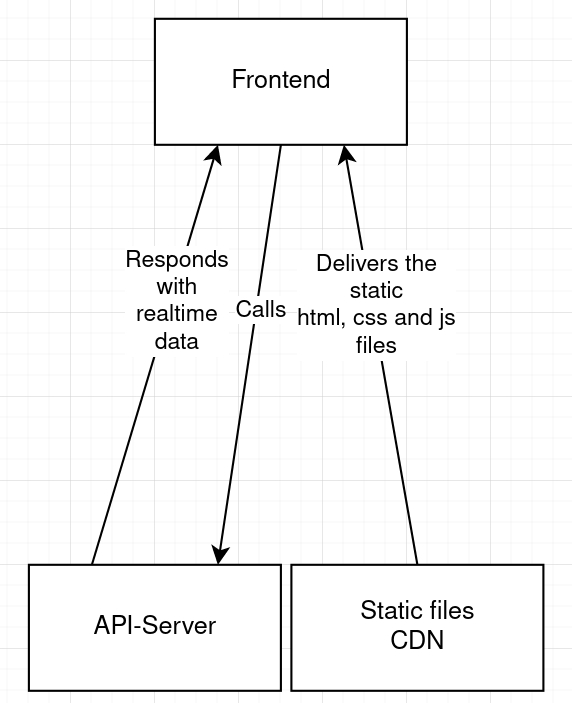
\includegraphics[width=\linewidth]{architecture.jpeg}
    \caption{Basic architecture}
\end{figure}
The separation between the API Server itself and the server that delivers the static files (html, css and js files) ensures that making changes, when the solution is running in production, is easy since the logic is separeted from the frontend and how it looks. If I would use a Backend that delivers the static files and does the logic as well it wouldn't scale well if you had to deploy it on more servers to balance the load. Additionally this ensures that you can have different frontends (mobile app and website for example) that have the same logic without having to implement it twice. Another pro for this architecture is that you could have different CDNs so that you get the static files form the geographical nearest CDN with increases the load speed.

\subsection{UI}
% TODO
Describe how to design the UI
\subsection{Backend-Endpoints}
I intend to build the backend in the programming language Python 3.9 using the Framework \href{https://fastapi.tiangolo.com/}{FastAPI} for building the backend. All needed python libraries will be installed and managed by pipenv since python library dependicies can be very difficult to resolve by hand and installing the libraries globally on your system might work on your machine but will cause issues once you deploy it.

The Backend should accept requests by the clients, fetch the nearest petrol stations from the \href{https://creativecommons.tankerkoenig.de/}{Tankerkönig API}, loop over the results, fetch the navigation instructions from the \href{https://developers.google.com/maps/documentation/directions/start}{Google Maps Directions API} and the \href{https://developers.google.com/maps/documentation/roads/overview}{Google Maps Roads API} 
% TODO: https://developer.here.com/pricing This might be an alternative for route calculations https://developer.here.com/documentation/routing/dev_guide/topics/resource-param-type-vehicle-type.html and https://developers.google.com/maps/documentation/distance-matrix/overview
 for each petrol station, calculate roughly how much fuel you would consume to get there from your current location and then sort it by cheapest. This would then be served to the clients. 

\section{Development}
\end{document}